\documentclass[12pt]{article}

\usepackage{styles/sbc-template}
\usepackage{graphicx,url}
\usepackage[utf8]{inputenc}
\usepackage[american]{babel}
% two images, same frame, side by side
\usepackage{subfig}
\usepackage{booktabs}
\usepackage{soul}
\usepackage{xcolor}
\usepackage{mdframed}
\usepackage{todonotes}

\sloppy

\title{Exploring the Energy Flow Classifier to Identify \\ Fraudulent Cryptocurrency Transactions}

\author{Kevin S. Araujo\inst{1}, Rodrigo Bonifacio de Almeida\inst{1}, \\ Fabiano Cavalcanti Fernandes\inst{2}, Joao Jose
Costa Gondim\inst{1}, Camila Pontes\inst{1}}
\address{Departamento de Ciências da Computação \\ -- Universidade de Brasília (UnB) \\ Campus Universitário Darcy Ribeiro,
Brasília-DF \nextinstitute Instituto Federal de Brasília (IFB) -- Taguatinga, DF -- Brazil \email{kevin.araujo@aluno.unb.br, 
rbonifacio@unb.br, fabiano.fernandes@ifb.edu.br} \email{gondim@unb.br, cftpontes@gmail.com}}


\newmdenv[
  backgroundcolor=gray!10,
  linecolor=gray!50,
  linewidth=1pt,
  roundcorner=5pt,
  skipabove=12pt,
  skipbelow=12pt,
  innertopmargin=6pt,
  innerbottommargin=6pt,
  innerleftmargin=10pt,
  innerrightmargin=10pt,
  frametitle=Takeaway,
  frametitlefont=\bfseries,
  frametitlebackgroundcolor=gray!20
]{highlightbox}

\begin{document} 

\maketitle

\begin{abstract}
  Fraudulent cryptocurrency transactions represent an ongoing and significant threat within the digital asset ecosystem,
  demanding robust detection mechanisms. Identifying such illicit activities is complicated by the complex nature of transaction
  data and, critically, the prevalent scarcity of labeled illicit examples in available datasets. This paper conducts a
  comprehensive empirical evaluation of the Energy Flow Classifier (EFC), a physics-inspired one-class anomaly detection
  model, for identifying illicit Bitcoin transactions using the Elliptic dataset, specifically addressing its performance
  under conditions of label scarcity. Our findings demonstrate that EFC can effectively distinguish illicit from licit
  transactions when trained exclusively on normal data, with its performance significantly enhanced by combining feature
  selection and data balancing techniques like SMOTE, achieving strong results even on imbalanced test sets.
\end{abstract}

\section{Introduction} \label{sec:introduction}
Bitcoin is an electronic transaction system that operates without a third-party moderator~\cite{nakamoto2008bitcoin}. It is
built on blockchain technology, where an immutable ledger of financial transactions is maintained through mathematics,
programming, and advanced cryptography. This distributed ledger architecture eliminates the need for central authorities
to establish trust. Although Bitcoin was designed to circumvent vulnerabilities in the traditional financial system
\cite{nakamoto2008bitcoin}, it is not immune to manipulation and anomalous activities and demands a robust detection
mechanisms~\cite{fang2022cryptocurrency, zhang2020financial,zainal2018review}. 

In fact, crypto-related fraud has become a significant threat, causing substantial financial losses and destroying
trust in the digital asset ecosystem. In 2023, for example, illicit addresses received \$24.2 billion in cryptocurrency,
indicating the scale of financial losses from scams, stolen funds, and other illicit activities \cite{chainalysis2024cryptocrime}.
These activities not only cause direct monetary damage to individuals and institutions, but also have broader implications,
such as undermining the legitimacy of cryptocurrency markets and hindering the widespread adoption of blockchain technology.
The need to develop effective methods for detecting and preventing cryptocurrency fraud is crucial to protect participants,
maintain market integrity, and ensure sustainable growth of the cryptocurrency industry \cite{scharfman2024, Khiari2025}.

However, detecting anomalous patterns within the intricate data streams of cryptocurrency transactions poses a significant
challenge. Like many modern datasets, these transactions are characterized by high dimensionality, evolving characteristics,
and substantial volume, which complicates the application of traditional anomaly detection methods. In this context, the
Energy-Based Flow Classifier (EFC) presents a promising approach rooted in statistical physics. Originally formulated using
the Inverse Potts model \cite{pontes2019}, the EFC characterizes the probability distribution of normal data flows through
an energy function derived from observed data patterns \cite{pontes2019}. Previous research has demonstrated the utility
of EFC in classifying unusual network traffic, suggesting its potential to adapt to detect fraudulent activity within cryptocurrency
systems \cite{pontes2019, souza2022novelopensetenergybased}. Its selection for this study is further motivated by its relatively
low computational complexity during both training and inference phases, rendering it a suitable candidate for real-time detection
applications where swift identification of illicit activities is paramount.

Building upon the promise of the Energy-Based Flow Classifier (EFC) framework, this paper presents a comprehensive empirical
evaluation of its application to the detection of illicit Bitcoin transactions. To this end, we first replicate a previous
study that employs machine learning algorithms such as K-Nearest Neighbors, One-Class Support Vector Machine, and Isolation
Forest for anomaly detection on the Elliptic dataset \footnote{Available at https://www.kaggle.com/ellipticco/elliptic-data-set}.
We then investigated the use of EFC as a potential alternative to these machine learning approaches, using the same data set
for consistency. Our findings confirm the EFC's ability to distinguish between licit and illicit transaction patterns based
on their energy profiles, showing strong performance in identifying illegal activity even when trained solely on licit data.
However, the results also highlight the critical sensitivity to specific configuration parameters. In particular, we observe
significant trade-offs between maximizing the detection rate of illicit transactions (recall) and minimizing false positives
(precision), especially concerning the energy threshold that defines anomalous behavior. 

Addressing the significant challenge of label scarcity inherent in datasets like Elliptic is crucial for developing effective
fraud detection systems. Traditional supervised machine learning methods often struggle in such scenarios due to the limited
availability of labeled illicit examples. This motivates the exploration of alternative approaches, particularly those capable
of learning from predominantly normal data. The Energy-based Flow Classifier (EFC) also emerges as a promising candidate
in this regard. Originally proposed for network intrusion detection \cite{pontes2019, souza2022novelopensetenergybased},
EFC was designed specifically to address key limitations of conventional ML classifiers, including the reliance on extensive
labeled datasets. A core strength highlighted in its foundational work is its ability to function as an anomaly-based classifier,
inferring a statistical model of normal behavior using only labeled *benign* (or licit, in our context) examples
\cite{souza2022novelopensetenergybased}. Deviations from this learned norm, characterized by higher 'energy' scores, are
then flagged as potential anomalies. This one-class learning paradigm directly tackles the label scarcity issue prevalent
in the Elliptic dataset, allowing us to model legitimate transaction patterns effectively even with few confirmed illicit
instances. Furthermore, EFC's demonstrated adaptability across different data distributions in network traffic analysis
suggests potential robustness in the dynamic environment of cryptocurrency transactions. Consequently, this paper evaluates
the suitability and performance of EFC for identifying illicit Bitcoin transactions by leveraging its capacity to model
normality from available licit data.

In summary, the main contributions of this paper are:

\begin{itemize}
    \item Novel Application and Empirical Evaluation of EFC for One-Class Bitcoin Anomaly Detection;
    \item In-depth analysis of the impact of data balancing and feature selection techniques on EFC's efficacy for
    identifying illicit transactions;
    \item Demonstration of a combined feature selection and data balancing (SMOTE) strategy as a robust approach for enhancing
    EFC performance on imbalanced cryptocurrency datasets.
\end{itemize}

\section{Background and Related Work} \label{sec:background}
Cryptocurrency manipulation involves deceptive strategies by individuals or groups to artificially distort market prices
for illicit profit \cite{cryptocurrency_arket_manipulation_2021}. Common tactics include pump-and-dump schemes (artificial
price inflation and subsequent sell-off) and wash trading (creating false trading volume) \cite{karim2018manipulation,
gandal2018price, edelman2018detecting}. The decentralized and pseudonymous nature of many platforms complicates the detection
of such activities, making robust detection mechanisms crucial.

The Energy-based Flow Classifier (EFC), rooted in statistical physics and initially applied to network traffic analysis
\cite{pontes2019}, offers a promising approach for identifying anomalous financial transactions. EFC assigns an "energy"
score to data points, where normal, expected patterns correspond to low-energy states, and significant deviations (potential
anomalies) manifest as high-energy states. This model is particularly suited for detecting anomalous Bitcoin transactions
due to its one-class learning capability; it can learn the characteristics of normal (Licit) behavior from predominantly
normal or unlabeled data, thereby addressing the common challenge of label scarcity in fraud datasets like Elliptic
\cite{bansal2022systematic}. Furthermore, EFC's energy function provides a holistic measure derived from multiple features,
potentially capturing complex, subtle deviations that simpler methods might miss \cite{wilson2024future}, and its prior
success in analogous domains suggests its utility for Bitcoin \cite{pontes2019, souza2022novelopensetenergybased}.

\section{Study Settings} \label{sec:methods}
This section details the data and methods employed in our study, which builds upon the foundational research presented
by \cite{lorenz2021machinelearningmethodsdetect}. That work explored the use of various machine learning classifiers (e.g.,
Random Forest, SVM, MLP) applied to engineered features from the Elliptic dataset to identify illicit Bitcoin transactions,
specifically tackling the inherent challenge of label scarcity. While demonstrating the potential of standard ML techniques,
their approach relied on supervised or semi-supervised algorithms requiring at least some labels. Our research
diverges by investigating the Energy Flow Classifier (EFC). 

\subsection{Dataset Description} \label{subsec:dataset}
This study uses the Elliptic dataset, a publicly available graph dataset of Bitcoin transactions introduced by 
\cite{weber2019antimoneylaunderingbitcoinexperimenting} and subsequently used in foundational studies on machine
learning for Bitcoin money laundering detection, including the work by~\cite{lorenz2021machinelearningmethodsdetect}
which highlighted the challenges of label scarcity in the Elliptic dataset. The dataset represents a temporal subgraph of
the public Bitcoin blockchain, focusing on transactions involving entities identified by Elliptic Ltd., a company specializing
in blockchain analytics and financial crime prevention. It captures transaction patterns over 49 distinct time steps, where
each step corresponds roughly to a two-week period. The full dataset comprises 203,769 transaction nodes and 234,355 directed edges
representing the flow of Bitcoin between transactions.

Each transaction (node) in the graph is described by a set of 166 anonymized features. One feature explicitly denotes the
time step (1 to 49). The remaining 165 features are local transactional properties, including aggregated information about
the transaction's inputs and outputs (e.g., number, amounts, fees) and potentially aggregated statistics from its immediate
neighborhood in the transaction graph. These features are provided in a normalized or standardized form, obscuring raw
values but preserving relational patterns crucial for machine learning analysis. The graph structure itself, defined by
the edges connecting transactions where the output of one becomes the input of another, provides contextual information
about the flow of funds---although our EFC implementation primarily focuses on the node features. A key characteristic of
the Elliptic dataset is its label scarcity---while the entire dataset contains over 200,000 transactions, only a subset of
46,564 transactions is explicitly labeled. This represents a central challenge addressed by \cite{lorenz2021machinelearningmethodsdetect}
and serves as a motivation for exploring EFC in this domain.  
The labels classify transactions into two main categories: (a) {\bf Licit Transactions} are those associated with known
legitimate entities such as exchanges, miners, wallet providers, and other regulated services (42,019 instances in the
original labeled set); and (b) {\bf Illicit Transactions} are linked to known illicit activities, including scams, ransomware,
terrorist financing, ponzi schemes, and dark market operations (4,545 instances in the original labeled set). Table~\ref{tab:dataset_summary}
summarizes the Elliptic dataset.

\begin{table}[htbp]
  \centering
  \caption{Summary Statistics of the Elliptic Dataset (based on \cite{weber2019antimoneylaunderingbitcoinexperimenting}).}
  \label{tab:dataset_summary}
  \begin{small}
  \begin{tabular}{lr}\toprule
    Characteristic        & Value \\ \midrule
    Total of Transactions (Nodes) & 203,769 \\
    Total of Edges           & 234,355 \\
    Time Steps            & 49 \\
    Features per Node     & 166 \\
    Labeled Transactions  & 46,564 (\textasciitilde23\%) \\
    \quad - Licit         & 42,019 (\textasciitilde90.2\% of labeled) \\
    \quad - Illicit       & 4,545 (\textasciitilde9.8\% of labeled) \\
    Unlabeled Transactions & 157,205 (\textasciitilde77\%) \\ \bottomrule
  \end{tabular}
  \end{small}
\end{table}

\subsection{Data Preprocessing} \label{subsec:preprocessing}
Preparing the Elliptic dataset for EFC involved several key steps focused on handling labels, selecting relevant features,
scaling the data appropriately, and partitioning it for training and evaluation in a temporally meaningful way.

To prepare the Elliptic dataset, we filtered transactions based on their assigned labels. Since the
EFC model learns patterns from \textit{normal} data to detect anomalies, transactions labeled as \textit{Licit} were used
as the normal class for training. In contrast, transactions labeled as \textit{Illicit} were treated as anomalies and reserved
for evaluation. Transactions with \textit{Unknown} labels were excluded from both training and testing to ensure that the
evaluation relied solely on transactions with a known ground truth. For the binary classification task (\textit{licit} vs.
\textit{illicit}), labels were mapped to numerical values---that is, value 0 for licit and value 1 for illicit.

We also performed feature selection and transformation. Of the 166 features available for each transaction, the feature
explicitly indicating the time step (ranging from 1 to 49) was removed. While this temporal information was essential for
partitioning the data in training and testing sets, it was excluded from the EFC model's input, as the model focuses on
intrinsic transaction properties rather than absolute temporal position. The remaining 165 anonymized features---representing
transactional and local graph characteristics---were retained as inputs to the EFC. Although the original dataset description
reports some form of normalization~\cite{weber2019antimoneylaunderingbitcoinexperimenting}, we decided to apply the Min-Max
scaling to the [0, 1] range to ensure consistency and enhance the stability of energy calculations within the EFC framework.
Scaling was applied separately to the training and test sets, with the scaler fitted exclusively on the training data to
prevent data leakage.

Finally, we implemented a temporal data split, in line with common practice for this dataset 
\cite{weber2019antimoneylaunderingbitcoinexperimenting, lorenz2021machinelearningmethodsdetect}, to simulate a realistic
scenario in which a model trained on historical data is used to detect fraudulent activity in future transactions.
Transactions from time steps 1 to 34 were allocated to the training set, while those from time steps 35 to 49 were reserved
for testing. The EFC model was trained exclusively on licit (normal) transactions from the training period (time steps 1-34).
The test set (time steps 35-49) included both licit and illicit transactions, enabling an evaluation of the model's ability
to assign higher energy scores to previously unseen illicit transactions compared to unseen licit ones.

\subsection{Energy Flow Classifier Configuration} \label{subsec:efc_implementation}

For detecting illicit transactions within the Elliptic dataset, we employed the Energy Flow Classifier (EFC), leveraging
the Python package implementation \cite{efc_package_github} based on the recommendations by Pontes et al.
\cite{pontes2019,souza2022novelopensetenergybased}. EFC operates on the premise that normal system behavior corresponds
to low-energy states, while anomalies or deviations manifest as high-energy states. Our implementation specifically
utilizes EFC as a one-class anomaly detector, tailored to the label scarcity challenge inherent in the Elliptic dataset.

To set up EFC in our experiment, we extended the class-based interface provided by the EFC Python package, specifically
by overriding the \texttt{EnergyBasedFlowClassifier} class to tailor its behavior to our evaluation needs. In our implementation,
we configured three key EFC hyperparameters: \texttt{n\_bins}, \texttt{cutoff\_quantile}, and \texttt{pseudocounts}.
The \texttt{n\_bins} parameter controls the discretization of input features, dividing each feature's range into a specified
number of bins. These bins form the basis for estimating state probabilities and computing energy values. Based on preliminary
experiments, we used \texttt{n\_bins = 30}. The \texttt{cutoff\_quantile} parameter sets the anomaly
threshold by determining the energy value corresponding to a quantile of the training data's energy distribution. For instance,
a setting of \texttt{cutoff\_quantile = 0.90} classifies any sample with an energy score above the 90th percentile as anomalous.
Finally, \texttt{pseudocounts} addresses the issue of zero probabilities when encountering states not seen in the training
data. We used a small \texttt{pseudocounts} of \texttt{0.10} to ensure numerical stability during energy computation.

Regarding the \emph{training process}, a central aspect of our EFC configuration is its alignment with the anomaly detection
setting under label scarcity. As outlined in Section~\ref{subsec:preprocessing}, the EFC model was trained exclusively on
licit (normal) transactions from the training period (time steps 1--34) by invoking its \texttt{fit} method. This follows
the one-class classification paradigm, in which the model learns the energy landscape associated with legitimate Bitcoin
transactions based solely on verified normal examples. Illicit transactions were entirely excluded from the training phase
to preserve the model's ability to generalize and detect anomalies without prior exposure to them.

During the evaluation phase, the trained EFC model's \texttt{predict} method was applied to the test set---transactions
from time steps 35--49, which contained both licit and illicit instances. For each test transaction, the EFC computed an
energy score based on its features and the probability distributions learned during training. If a transaction's energy
score exceeded the pre-determined cutoff threshold (derived from the \texttt{cutoff\_quantile} applied to the training data's
energy distribution), it was classified as anomalous (predicted illicit); otherwise, it was classified as normal (predicted licit).
The energy scores were also used to compute evaluation metrics such as AUC, which assess ranking performance rather than
relying on a fixed classification threshold.

\subsection{Research Characterization: Goal, Questions, and Metrics} \label{subsec:task}

The primary goal of this study is to evaluate the effectiveness of the Energy Flow Classifier (EFC), configured
as we discussed in Section \ref{subsec:efc_implementation}, for identifying illicit transactions within the Elliptic
Bitcoin dataset. This aligns with the broader goal of exploring alternative methodologies, particularly those suited for
label scarcity, compared to the supervised approaches examined by \cite{lorenz2021machinelearningmethodsdetect}. Our aim
is to answer the following research question: \emph{How effective is the Energy-Based Flow Classifier (EFC) under conditions
of label scarcity in identifying illicit transactions in the Elliptic Bitcoin dataset?}

Specifically, our research is thus framed as a \emph{one-class anomaly detection problem}. Having trained the EFC model exclusively
on Licit transactions from the initial time steps (1-34), the objective is to assess its ability to distinguish between
licit and illicit transactions in the subsequent, unseen time steps (35-49) of the test set. This evaluation involves
two main perspectives:

\begin{enumerate}
    \item \textbf{Classification Performance:} Using the energy threshold derived from the training data, based on the
      \texttt{cutoff\_quantile}, we assess how well EFC classifies unseen transactions as either licit (below threshold)
      or illicit (above threshold). Performance is measured using standard classification metrics suitable for imbalanced
      datasets, such as Precision, Recall, F1-Score, and potentially Balanced Accuracy, calculated on the labeled test set.
      
    \item \textbf{Ranking Performance:} Independent of a specific threshold, we evaluate EFC's ability to assign consistently
      higher energy scores to illicit transactions compared to licit transactions in the test set. This is primarily
      assessed using the Area Under the Receiver Operating Characteristic Curve (AUC-ROC), which measures the model's
      ability to rank anomalies higher than normal instances across all possible thresholds.
\end{enumerate}

The outcomes of this research provide insights into the potential of the EFC model as a viable tool for detecting fraudulent or
anomalous Bitcoin transactions. Its energy-based methodology is employed by primarily training on transactions labeled as
'licit'—those implicitly defined as normal due to the absence of reported fraud to establish a baseline of typical behavior
within a one-class learning framework. This approach allows EFC to address the scarcity of explicitly labeled illicit
examples and to identify novel deviations indicative of fraudulent activity.

Model performance was assessed using a combination of quantitative metrics and visual analysis. We use the \textbf{F1-Score
Macro Average} as the primary evaluation metric, following the same design decision of \cite{lorenz2021machinelearningmethodsdetect}.
This metric calculates the F1-score for each class (Licit and Illicit) independently and then averages them, providing a
balanced measure of performance across both classes, which is crucial given the inherent class imbalance. 
We also leverage \textbf{Specific Metrics for the Illicit Class}, since our primary interest lies in detecting anomalous
transactions. As such, we also report Precision, Recall, and the F1-Score specifically calculated for the Illicit class
based on the classification derived from the \texttt{cutoff\_quantile} threshold. These metrics offer direct insight into
the model's effectiveness in identifying illicit transactions and the associated trade-offs (e.g., false positives vs.
false negatives).  Finally, we highlight in plots the \textbf{EFC Energy Distributions.} For the experiments we detail in
the next section, we show histograms comparing the distribution of EFC energy scores assigned to Licit versus Illicit
transactions in the test set that were generated. These plots provide a visual assessment of the model's separation capability.

\section{Results} \label{sec:results}

This section presents the results from the application of the Energy Flow Classifier (EFC) to the task of
classifying illicit transactions within the Elliptic dataset. Following the settings outlined in Section
\ref{sec:methods}, we explore the EFC classifier primarily as a one-class anomaly detector, trained exclusively on transactions
labeled as Licit from the initial time steps (1-34). The core objective was to evaluate the model's capability to distinguish
these known Licit patterns from potentially anomalous Illicit transactions present in the unseen test set (time steps 35-49).
We evaluate performance based on the EFC's ability to assign distinct energy scores to the two classes, using
metrics appropriate for imbalanced anomaly detection scenarios. The following subsections detail the outcomes of three specific
experiments we conducted, focusing on data balancing, feature engineering/selection, and model comparison/tuning, respectively.
All experiments utilized the Elliptic dataset, preprocessed as described previously, employing a standard train-test split methodology.

\subsection{Experiment 1: Impact of Data Balancing Techniques} \label{subsec:experiment_1}

This experiment examined the impact of different data balancing strategies on classification performance using the inherently
imbalanced EFC dataset. We estimate the \emph{baseline performance} using the original, unbalanced dataset. 
This baseline was then compared against four widely
adopted balancing techniques, each applied to both the training and test datasets: (a) creating a balanced subset by undersampling
the majority class prior to the train-test split, (b) applying the Synthetic Minority Over-sampling Technique (SMOTE), (c)
performing random oversampling of the minority class, and (d) performing random undersampling of the majority class. To ensure
a fair comparison, the composition of the test set was kept consistent across most techniques. We evaluate model performance
using Accuracy, Precision, Recall, weighted F1-Score, Macro F1-Score, and confusion matrices. Table~\ref{tab:balancing_results}
and Figure~\ref{fig:histexp1} present a summary of the classification outcomes.

\begin{table}[htbp]
  \centering
  \caption{EFC Performance Across Data Balancing Techniques (Experiment 1).}
  \label{tab:balancing_results}
  \resizebox{\textwidth}{!}{
    \begin{tabular}{lrrrrrrrrr}
      \toprule
      \textbf{Configuration} & \textbf{TP} & \textbf{FN} & \textbf{FP} & \textbf{TN} & \textbf{Accuracy} & \textbf{Precision}
      & \textbf{Recall} & \textbf{F1-Score} & \textbf{F1-Macro} \\
      & & & & & & & & \textbf{(Weighted)} & \\
      \midrule
      Unbalanced Dataset (Baseline)$^{a}$ & 15117 & 470 & 1064 & 19 & 0.908 & 0.876 & 0.908 & 0.891 & 0.488 \\
      Balanced Dataset (Equally Dist.)$^{b}$ & 516 & 848 & 37 & 1326 & 0.675 & 0.772 & 0.675 & 0.644 & 0.644 \\
      SMOTE$^{b}$ & 10831 & 1775 & 530 & 12076 & 0.909 & 0.913 & 0.909 & 0.908 & \textbf{0.908} \\
      Random Oversampling$^{a}$ & 15393 & 194 & 1013 & 70 & 0.928 & 0.895 & 0.928 & 0.907 & 0.533 \\
      Random Undersampling$^{a}$ & 13791 & 1796 & 412 & 671 & 0.868 & 0.926 & 0.868 & 0.890 & 0.652 \\
      \bottomrule
    \end{tabular}
  }
  \par\medskip
  \footnotesize
  \textit{Note: TP=True Positives, FN=False Negatives, FP=False Positives, TN=True Negatives. Metrics are rounded. F1-Score
    is weighted average. F1-Macro for SMOTE is bolded as it's the highest among these techniques. Test set composition:
    ($^{a}$) Imbalanced, ($^{b}$) Balanced.}
\end{table}

\begin{figure}[!tph]
  \centering
  \subfloat[Unbalanced Dataset.]{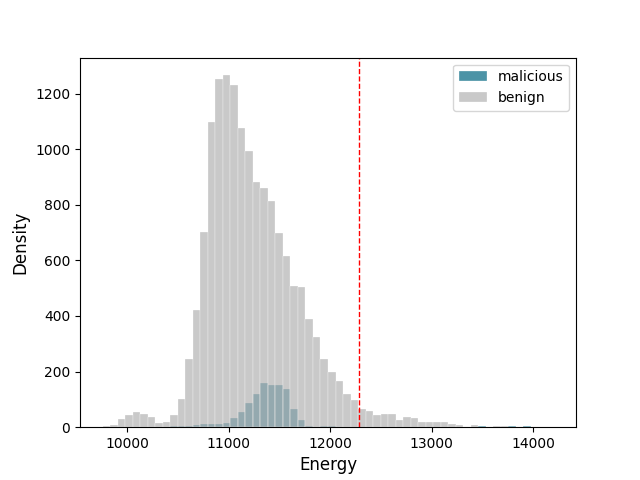
\includegraphics[width=0.35\textwidth]{figures/experiment-1/1_unbalanced_dataset.png}\label{fig1:1_unbalanced_dataset}}
  \subfloat[Balanced Dataset.]{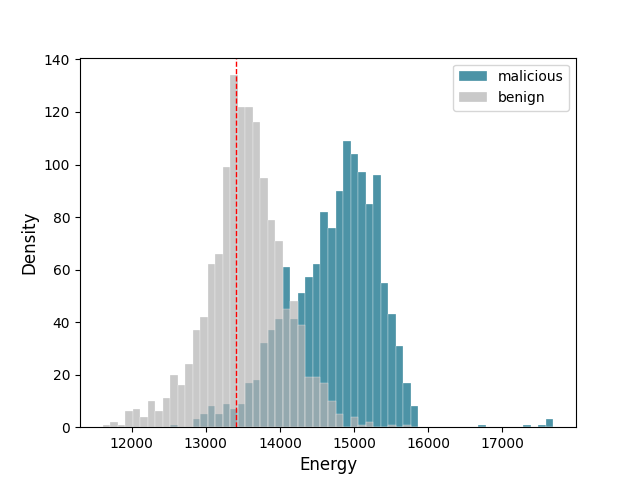
\includegraphics[width=0.35\textwidth]{figures/experiment-1/2_balaced_dataset.png}\label{fig2:2_balaced_dataset}}
  \subfloat[SMOTE.]{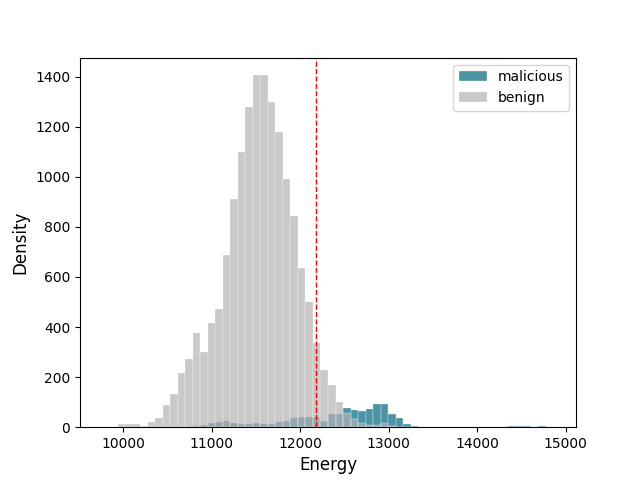
\includegraphics[width=0.35\textwidth]{figures/experiment-1/3_smote_minority_full_test_dataset.png}\label{fig3:3_smote_minority}}
  \caption{Experiment 1: Energy Distribution of Licit and Illicit Transactions.}
  \label{fig:histexp1}
\end{figure}

% \paragraph{Discussion of Experiment 1 Results}
The results from Experiment 1 (Table~\ref{tab:balancing_results}) clearly illustrate the EFC's sensitivity to class imbalance
and the significant impact of balancing techniques. The baseline ``Unbalanced Dataset,'' when tested on an imbalanced test
set, yielded a low F1-Macro score of 0.488, confirming the difficulty in detecting the minority illicit class without
intervention. This result is most likely due to the nature of one-class classifiers and imbalanced data. Applying SMOTE
and evaluating on a balanced test set resulted in a striking improvement, with an F1-Macro of 0.908. This suggests that
EFC can perform exceptionally well if the training data is appropriately balanced and the evaluation scenario also reflects
a more balanced class distribution. 

Other techniques applied to the training data but evaluated on an imbalanced test set
also showed improvements over the baseline: Random Oversampling achieved an F1-Macro of 0.533, and Random Undersampling
reached 0.652. This indicates that even simpler balancing methods can enhance EFC's performance on imbalanced test data,
with undersampling being more effective than oversampling in this specific setup. The ``Balanced Dataset (Equally Dist.)''
technique, which involved undersampling the majority class to create a balanced training and test set, achieved an F1-Macro
of 0.644. While better than the baseline, it did not match SMOTE's performance on a balanced test set, suggesting that
SMOTE's approach of generating synthetic minority samples is more beneficial for EFC in such conditions. 

\begin{highlightbox}
The stark contrast in F1-Macro scores, particularly between SMOTE on a balanced test set and other techniques on imbalanced
test sets, underscores the critical influence of test set composition on this metric.
\end{highlightbox}

\subsection{Experiment 2: Impact of Feature Selection} \label{subsec:experiment_2}

Following the analysis of data balancing, our second experiment focused on evaluating the impact of feature selection on
classification performance using the Energy-Based Flow Classifier (EFC). We employed the \texttt{SelectKBest} algorithm
(available in the scikit-learn library), utilizing the ANOVA F-value (\texttt{f\_classif}) scoring function to rank and
select features based on their relevance to the class labels. 

In this experiment, we systematically varied the number of selected features ($k$), testing values of $k \in \{10, 20, 30,
40, 50, 60\}$. We applied the feature selection process to the features and labels of the original unbalanced dataset
\textit{before} the standard train-test split was performed on the resulting (and smaller) feature set. Furthermore, we conducted
two distinct series of runs: one applying feature selection to the complete feature set, including aggregated temporal
features, and another applying it only to the raw node features after explicitly excluding the aggregated ones. This
decision was driven by the need to understand the specific impact and contribution of these aggregated features. 

Aggregated features, which represent statistical summaries of a node's neighborhood, often possess high individual predictive
power due to the condensed information they carry about local graph structure. Including these potentially dominant features
in the \texttt{SelectKBest} algorithm ({\bf Scenario 1}) could lead to them consistently ranking highest, potentially masking
the predictive contribution of the node's intrinsic \cite{weber2019antimoneylaunderingbitcoinexperimenting}, raw features.
By running a separate scenario ({\bf Scenario 2}) where these aggregated features were removed \textit{before} applying
\texttt{SelectKBest}, we aimed to isolate and evaluate the predictive capability derived solely from the raw node characteristics.
This allows for a clearer comparison and a better understanding of which feature types (raw vs. aggregated) are most crucial
for classification, especially when operating under the dimensionality constraints imposed by selecting only the top $k$ features.

Performance for each value of $k$ and for both feature set scenarios (with and without aggregated features) was assessed
using standard classification metrics (Accuracy, Precision, Recall, F1-Score, and F1-Macro). The objective was to
determine if reducing dimensionality could maintain or improve the EFC performance on correctly classifying illicit transactions,
identify an optimal number of features ($k$), and understand the contribution of aggregated features within this selection context.
We summarize the results in Table~\ref{tab:fs_excluded_agg_results} (Scenario 1) Table~\ref{tab:fs_included_agg_results} (Scenario 2).
Considering both scenarios, a key observation is that EFC can achieve its best performance with a significantly reduced
feature set. When aggregated features were excluded (Table~\ref{tab:fs_excluded_agg_results}), the highest F1-Macro score
of 0.686 was obtained with only $k=10$ features. Similarly, when aggregated features were included in the selection pool
(Table~\ref{tab:fs_included_agg_results}), the peak F1-Macro was 0.689, also at $k=10$.


\begin{table}[htb]
  \centering
  \caption{EFC Performance with Feature Selection (Aggregated Features Excluded) for Varying k (Experiment 2 - Scenario 1).}
  \label{tab:fs_excluded_agg_results}
  \resizebox{\textwidth}{!}{
  \begin{tabular}{lrrrrrrrrr}
    \hline
    \textbf{k Value} & \textbf{TP} & \textbf{FN} & \textbf{FP} & \textbf{TN} & \textbf{Accuracy} & \textbf{Precision} & \textbf{Recall} & \textbf{F1-Score} & \textbf{F1-Macro} \\
    & & & & & & & & \textbf{(Weighted)} & \\
    \hline
    10 & 11317 & 1289 & 598 & 766 & 0.865 & 0.893 & 0.865 & 0.877 & \textbf{0.686} \\
    20 & 11326 & 1280 & 859 & 505 & 0.847 & 0.866 & 0.847 & 0.856 & 0.617 \\
    30 & 11330 & 1276 & 1103 & 261 & 0.830 & 0.839 & 0.830 & 0.834 & 0.542 \\
    40 & 11305 & 1301 & 1341 & 23  & 0.811 & 0.808 & 0.811 & 0.810 & 0.456 \\
    50 & 11291 & 1315 & 1318 & 46  & 0.812 & 0.811 & 0.812 & 0.811 & 0.465 \\
    60 & 11254 & 1352 & 1138 & 226 & 0.822 & 0.833 & 0.822 & 0.827 & 0.527 \\
    \hline
  \end{tabular}
  }
  \par\medskip
  \footnotesize
  \textit{Note: Feature selection excluding aggregated features. TP=True Positives, FN=False Negatives, FP=False Positives,
  TN=True Negatives. Metrics rounded to three decimal places. F1-Score is weighted average. F1-Macro for k=10 is bolded
  as it's the highest.}
\end{table}

\begin{table}[htb]
  \centering
  \caption{EFC Performance with Feature Selection (Aggregated Features Included) for Varying k (Experiment 2 - Scenario 2).}
  \label{tab:fs_included_agg_results}
  \resizebox{\textwidth}{!}{
  \begin{tabular}{lrrrrrrrrr}
    \hline
    \textbf{k Value} & \textbf{TP} & \textbf{FN} & \textbf{FP} & \textbf{TN} & \textbf{Accuracy} & \textbf{Precision} & \textbf{Recall} & \textbf{F1-Score} & \textbf{F1-Macro} \\
    & & & & & & & & \textbf{(Weighted)} & \\
    \hline
    10 & 11254 & 1352 & 560 & 804 & 0.863 & 0.896 & 0.863 & 0.876 & \textbf{0.689} \\
    20 & 11297 & 1309 & 656 & 708 & 0.859 & 0.887 & 0.859 & 0.871 & 0.669 \\
    30 & 11309 & 1297 & 789 & 575 & 0.851 & 0.874 & 0.851 & 0.861 & 0.635 \\
    40 & 11296 & 1310 & 991 & 373 & 0.835 & 0.851 & 0.835 & 0.843 & 0.576 \\
    50 & 11291 & 1315 & 1265 & 99  & 0.815 & 0.818 & 0.815 & 0.817 & 0.484 \\
    60 & 11269 & 1337 & 1261 & 103 & 0.814 & 0.819 & 0.814 & 0.816 & 0.485 \\
    \hline
  \end{tabular}
  }
  \par\medskip
  \footnotesize
  \textit{Note: Feature selection including aggregated features. TP=True Positives, FN=False Negatives, FP=False Positives,
  TN=True Negatives. Metrics rounded to three decimal places. F1-Score is weighted average. F1-Macro for k=10 is bolded
  as it's the highest.}
\end{table}

This suggests that a small subset of the most relevant features suffices for EFC, and including more beyond the optimal $k$
(typically $k>20$) tends to degrade performance, likely due to noise or less informative features affecting EFC's energy
calculations. This diminishing return is a common pattern in feature selection. The slightly higher F1-Macro observed with
aggregated features (0.689 vs. 0.686) highlights their predictive value, even when only a few are selected. Still, the feature
engineering procedures in this second experiment did not match the performance achieved with the SMOTE data balancing technique,
which reached an F1-Macro of 0.908 on a balanced test set.

\begin{highlightbox}
While feature selection is beneficial for dimensionality reduction and can improve upon the baseline,
addressing class imbalance appears to be a more critical factor for enhancing EFC's F1-Macro score in the Elliptic dataset.
Still, the results confirm that feature selection can be effective, but might not be a complete solution without tackling imbalance.
\end{highlightbox}

\subsection{Experiment 3: Combining Feature Selection and Data Balancing} \label{subsec:experiment_3}

The goal of this third experiment is to investigate the combined impact of feature selection and data balancing on the
performance of the EFC classifier. It builds upon the findings of Experiment~1 (data balancing) and Experiment~2
(feature selection). The central idea is to first reduce the dataset's dimensionality using the feature selection method
identified in Experiment~2, and then apply the SMOTE balancing technique (from Experiment~1) to the reduced training data
before training the EFC model.

In more detail, for each value of $k \in \{10, 20, 30, 40, 50, 60\}$, we applied the \texttt{SelectKBest} algorithm with
the \texttt{f\_classif} scoring function to the original, unbalanced dataset---following the approach used in the first
scenario of Experiment~2---to retain only the top $k$ features. This $k$-feature dataset was then subjected to the SMOTE
procedure. Specifically, we first split the dataset into training and test sets. Next, we applied SMOTE to the training
set to balance the class distribution. The EFC classifier was then trained on this balanced, feature-reduced training data,
and evaluated on the corresponding unbalanced test set (which contained the same $k$ selected features).
We evaluated the performance using standard classification metrics (again, Accuracy, Precision, Recall, F1-Score, and Macro
F1-Score). This evaluation aimed to determine whether applying feature selection before SMOTE could lead to improved
classification performance, compared to using SMOTE on the full feature set (as in Experiment~1) or applying feature
selection alone (as in Experiment~2).

We summarize the results in Table~\ref{tab:exp3_smote_fs_results} (Experiment 3a, standard unbalanced test set) and
Table~\ref{tab:exp3_smote_fs_full_test_results} (Experiment 3b, ``Full Test Dataset'' context, also using an unbalanced test set). 
In Experiment 3a, the combination yielded a peak F1-Macro score of 0.808 when $k=30$ features were selected before applying
SMOTE. This is a substantial improvement compared to using feature selection alone (Experiment 2, best F1-Macro ~0.689)
and the baseline (0.488). It also surpasses the F1-Macro achieved by Random Undersampling alone (0.652) on a similar imbalanced
test set. That is, combining two effective strategies---dimensionality reduction to focus on salient features and SMOTE to
address imbalance---leads to an improvement in the overall performance. The optimal $k=30$ here is higher than the $k=10$
found in Experiment 2, though, suggesting that SMOTE might benefit from a slightly richer, yet still reduced, feature
set to generate more effective synthetic samples. 

Experiment 3b, conducted under the ``Full Test Dataset'' context (which also utilized an imbalanced test set as per its
note), showed a similar trend, with $k=30$ also yielding the best F1-Macro score of 0.770. While this is still a significant
improvement over the baseline and feature selection alone, it is slightly lower than the 0.808 achieved in Experiment 3a.
This discrepancy, despite both experiments testing on imbalanced sets, could be attributed to subtle differences in the
exact composition or characteristics of the test data partitions used, or slight variations in the feature subsets selected
if the ``Full Test Dataset'' context implied any nuanced differences in the overall feature pool available before selection
for that specific run. Overall, Experiment 3 shows that a combined strategy of feature selection followed by SMOTE balancing is highly
effective for improving EFC's F1-Macro score on imbalanced test data, outperforming either technique applied in isolation
(when FS is tested on imbalanced data). 

\begin{highlightbox}
Even when combining feature selection with SMOTE, the F1-Macro score remains below the 0.908 achieved by SMOTE alone on
a balanced test set---underscoring the dominant influence of test set composition on this metric.
\end{highlightbox}


\begin{table*}[htb]
  \centering
  \caption{EFC Performance: SMOTE with Feature Selection for Varying k (Experiment 3a).}
  \label{tab:exp3_smote_fs_results}
  \resizebox{\textwidth}{!}{
  \begin{tabular}{lrrrrrrrrr}
    \hline
    \textbf{k Value} & \textbf{TP} & \textbf{FN} & \textbf{FP} & \textbf{TN} & \textbf{Accuracy} & \textbf{Precision} & \textbf{Recall} & \textbf{F1-Score} & \textbf{F1-Macro} \\
    & & & & & & & & \textbf{(Weighted)} & \\
    \hline
    10 & 11319 & 1287 & 369 & 995 & 0.891 & 0.931 & 0.891 & 0.891 & 0.770 \\
    20 & 11326 & 1280 & 263 & 1101 & 0.900 & 0.939 & 0.900 & 0.900 & 0.798 \\
    30 & 11331 & 1275 & 226 & 1138 & 0.903 & 0.942 & 0.903 & 0.903 & \textbf{0.808} \\
    40 & 11272 & 1334 & 223 & 1141 & 0.900 & 0.940 & 0.900 & 0.900 & 0.799 \\
    50 & 11233 & 1373 & 247 & 1117 & 0.894 & 0.935 & 0.894 & 0.894 & 0.780 \\
    60 & 11239 & 1367 & 243 & 1121 & 0.895 & 0.936 & 0.895 & 0.895 & 0.783 \\
    \hline
  \end{tabular}
  }
  \par\medskip
  \footnotesize
  \textit{Note: SMOTE applied to training data after feature selection (including aggregated features). Test set is unbalanced.
  TP=True Positives, FN=False Negatives, FP=False Positives, TN=True Negatives. Metrics rounded. F1-Score is weighted average.
  F1-Macro for k=30 is bolded.}
\end{table*}

\begin{table*}[htb]
  \centering
  \caption{EFC Performance: SMOTE with Feature Selection (Full Test Dataset Context) for Varying k (Experiment 3b).}
  \label{tab:exp3_smote_fs_full_test_results}
  \resizebox{\textwidth}{!}{
  \begin{tabular}{lrrrrrrrrr}
    \hline
    \textbf{k Value} & \textbf{TP} & \textbf{FN} & \textbf{FP} & \textbf{TN} & \textbf{Accuracy} & \textbf{Precision} & \textbf{Recall} & \textbf{F1-Score} & \textbf{F1-Macro} \\
    & & & & & & & & \textbf{(Weighted)} & \\
    \hline
    10 & 11322 & 1284 & 368 & 996 & 0.882 & 0.894 & 0.882 & 0.917 & 0.739 \\
    20 & 11302 & 1304 & 259 & 1105 & 0.888 & 0.901 & 0.888 & 0.927 & 0.761 \\
    30 & 11313 & 1293 & 218 & 1146 & 0.892 & 0.905 & 0.892 & 0.931 & \textbf{0.770} \\
    40 & 11254 & 1352 & 222 & 1142 & 0.887 & 0.901 & 0.887 & 0.930 & 0.763 \\
    50 & 11258 & 1348 & 249 & 1115 & 0.886 & 0.899 & 0.886 & 0.927 & 0.758 \\
    60 & 11278 & 1328 & 249 & 1115 & 0.887 & 0.901 & 0.887 & 0.927 & 0.760 \\
    \hline
  \end{tabular}
  }
  \par\medskip
  \footnotesize
  \textit{Note: SMOTE applied to training data after feature selection (including aggregated features). Test set is unbalanced
  (1364 Malicious, 12606 Benign). TP=True Positives, FN=False Negatives, FP=False Positives, TN=True Negatives. Metrics rounded.
  F1-Score is weighted average. F1-Macro for k=30 is bolded.}
\end{table*}

\section{Discussion}
\label{sec:discussion}
In this section, we summarize the results of our three experiments by answering our research question Section~\ref{sec:answers}),
comparing them with the results of a previous work that explored active learning on the Elliptic Dataset~\cite{elliptic_dataset_kaggle}
(Section~\ref{sec:comparision}), and highlight some threats to validity that might compromise the generalization of our
findings (Section~\ref{sec:threats}).

\subsection{Answers to the Research Questions}\label{sec:answers}

The primary research question guiding this study was: \emph{How effective is the Energy-Based Flow Classifier (EFC) under
conditions of label scarcity in identifying illicit transactions in the Elliptic Bitcoin dataset?} Our experiments demonstrate
that EFC can be an effective algorithm, but its performance is critically dependent on addressing the inherent class imbalance
typical of fraud detection datasets. When trained solely on Licit transactions and applied to the raw, imbalanced dataset,
EFC's ability to distinguish the minority Illicit class was limited, yielding a low F1-Macro score of 0.488 (Experiment 1,
Baseline). This highlights that, in its basic one-class configuration, EFC struggles with severe imbalance.

For practical application on datasets (like the Elliptic dataset) where test data will likely remain imbalanced, we still
recommend researchers and pratitioners to combine Feature Selection and Data Balancing. In our settings, the best performance
on an imbalanced test set (F1-Macro 0.808) was achieved by first applying feature selection (e.g., \texttt{SelectKBest}
with $k \approx 30$ features, including aggregated ones) and then applying SMOTE to the reduced training dataset.
While SMOTE alone yielded a very high F1-Macro (0.908 in Experiment 1), this was under the condition of a \textit{balanced
test set}---a scenario that is often unrealistic for real-world fraud detection. When SMOTE alone is applied to the training
set and tested on an imbalanced set, its performance, while an improvement over no balancing, is surpassed by the combined
SMOTE and Feature Selection approach for imbalanced test scenarios.

\subsection{Comparison With Previous Work}\label{sec:comparision}
This study builds upon and diverges from previous research on detecting illicit Bitcoin transactions, in particular the
work by Lorenz et al.~\cite{lorenz2021machinelearningmethodsdetect}, which also utilized the Elliptic dataset and addressed the
challenge of label scarcity. Lorenz et al.~\cite{lorenz2021machinelearningmethodsdetect} explored various standard machine
learning classifiers, including Random Forests, SVMs, and MLPs, employing supervised or semi-supervised learning frameworks.
These approaches, while demonstrating potential, typically require a certain number of labels for both licit and illicit
classes, or sophisticated semi-supervised strategies to leverage unlabeled data.

Our research takes a different methodological path by investigating the Energy Flow Classifier (EFC), a physics-inspired
model rooted in statistical mechanics. Here we leverage the  \emph{One-Class Learning Paradigm}, since we trained the EFC
model \textit{exclusively} on Licit transactions. This directly addresses label scarcity by not requiring any Illicit labels
during the training phase, learning a model of ``normal'' behavior and identifying deviations. This contrasts with the
supervised/semi-supervised methods explored in previous research~\cite{lorenz2021machinelearningmethodsdetect}.
While Lorenz et al. demonstrated the utility of established ML techniques under label scarcity, our work explores EFC as
a novel alternative specifically suited for scenarios where only normal data is reliably labeled. The results, particularly
with SMOTE and feature selection (F1-Macro 0.808 on imbalanced test data), suggest EFC can be competitive. 

\subsection{Threats to Validity}\label{sec:threats}

Several factors may affect the validity and generalizability of our findings. First, we did not perform systematic hyperparameter
optimization of EFC, which may have limited its performance in some experiments. Second, while our temporal split (time
steps 1-34 for training, 35-49 for testing) follows a standard approach, it is only one possible strategy; alternative
splits could lead to different results. Similarly, our use of \texttt{SelectKBest} with the ANOVA F-value for feature
selection is just one technique---others may produce different feature subsets and outcomes.
Our analysis also depends on the quality of the labels provided in the Elliptic dataset; any label noise or bias could
impact both training and evaluation. Furthermore, the Elliptic dataset only includes anonymized features, which limits
interpretability and hinders domain-specific feature engineering. Finally, our conclusions are drawn exclusively from
the Elliptic dataset, and generalizing to other cryptocurrency transaction datasets or fraud detection scenarios warrants
further investigation.

\section{Conclusion} \label{section:conclusion}

This study investigated the Energy Flow Classifier (EFC) as a one-class anomaly detection method for identifying illicit
Bitcoin transactions within the Elliptic dataset, focusing on scenarios with label scarcity. In evaluating the performance of the
different techniques across our experiments, we adopted the \textbf{F1-macro score} as the primary overall metric. This
choice aligns with the methodology presented by \cite{lorenz2021machinelearningmethodsdetect} in their work on detecting
money laundering in Bitcoin, particularly relevant given the common challenge of label scarcity in such datasets.
The F1-macro score is calculated by first determining the F1 score (the harmonic mean of precision and recall) for each
individual class. Then, the unweighted average of these per-class F1 scores is taken. This approach ensures that each class
contributes equally to the final metric, regardless of its frequency in the dataset, providing a balanced assessment of
model performance, especially crucial in imbalanced scenarios like fraud detection where correctly identifying the minority
class is often of high importance.

The baseline performance of EFC on unbalanced data was modest in terms of distinguishing the minority Illicit class
(F1-Macro 0.488). However, we demonstrated that its effectiveness can be significantly enhanced through data preprocessing.
Specifically, applying the SMOTE balancing technique to the training data, especially when combined with feature selection
(reducing to $k \approx 30$ features), substantially improved the F1-Macro score to 0.808 when evaluated on a realistic,
imbalanced test set. This highlights that EFC can achieve robust performance if the data imbalance is appropriately managed.

In summary, EFC offers a valuable approach for one-class anomaly detection in cryptocurrency transactions due to its ability
to learn from only normal data. Its practical application, however, requires careful consideration of data preprocessing
strategies, notably class balancing and potentially feature selection, to optimize its detection capabilities for rare illicit
events.

\bibliographystyle{sbc}
\bibliography{bibliography/sbc-template.bib}

\end{document}
